\chapter{Design}
\label{sec:design}

% Ist das zentrale Kapitel der Arbeit. Hier werden das Ziel sowie die
% eigenen Ideen, Wertungen, Entwurfsentscheidungen vorgebracht. Es kann
% sich lohnen, verschiedene Möglichkeiten durchzuspielen und dann
% explizit zu begründen, warum man sich für eine bestimmte entschieden
% hat. Dieses Kapitel sollte - zumindest in Stichworten - schon bei den
% ersten Festlegungen eines Entwurfs skizziert werden.
% Es wird sich aber in einer normal verlaufenden
% Arbeit dauernd etwas daran ändern. Das Kapitel darf nicht zu
% detailliert werden, sonst langweilt sich der Leser. Es ist sehr
% wichtig, das richtige Abstraktionsniveau zu finden. Beim Verfassen
% sollte man auf die Wiederverwendbarkeit des Textes achten.

% Plant man eine Veröffentlichung aus der Arbeit zu machen, können von
% diesem Kapitel Teile genommen werden. Das Kapitel wird in der Regel
% wohl mindestens 8 Seiten haben, mehr als 20 können ein Hinweis darauf
% sein, daß das Abstraktionsniveau verfehlt wurde.

%\ldots design \ldots

%\todo{write design}

DESIGN





\subsection{k8s overview}

    \begin{figure}[H]
        \centering
        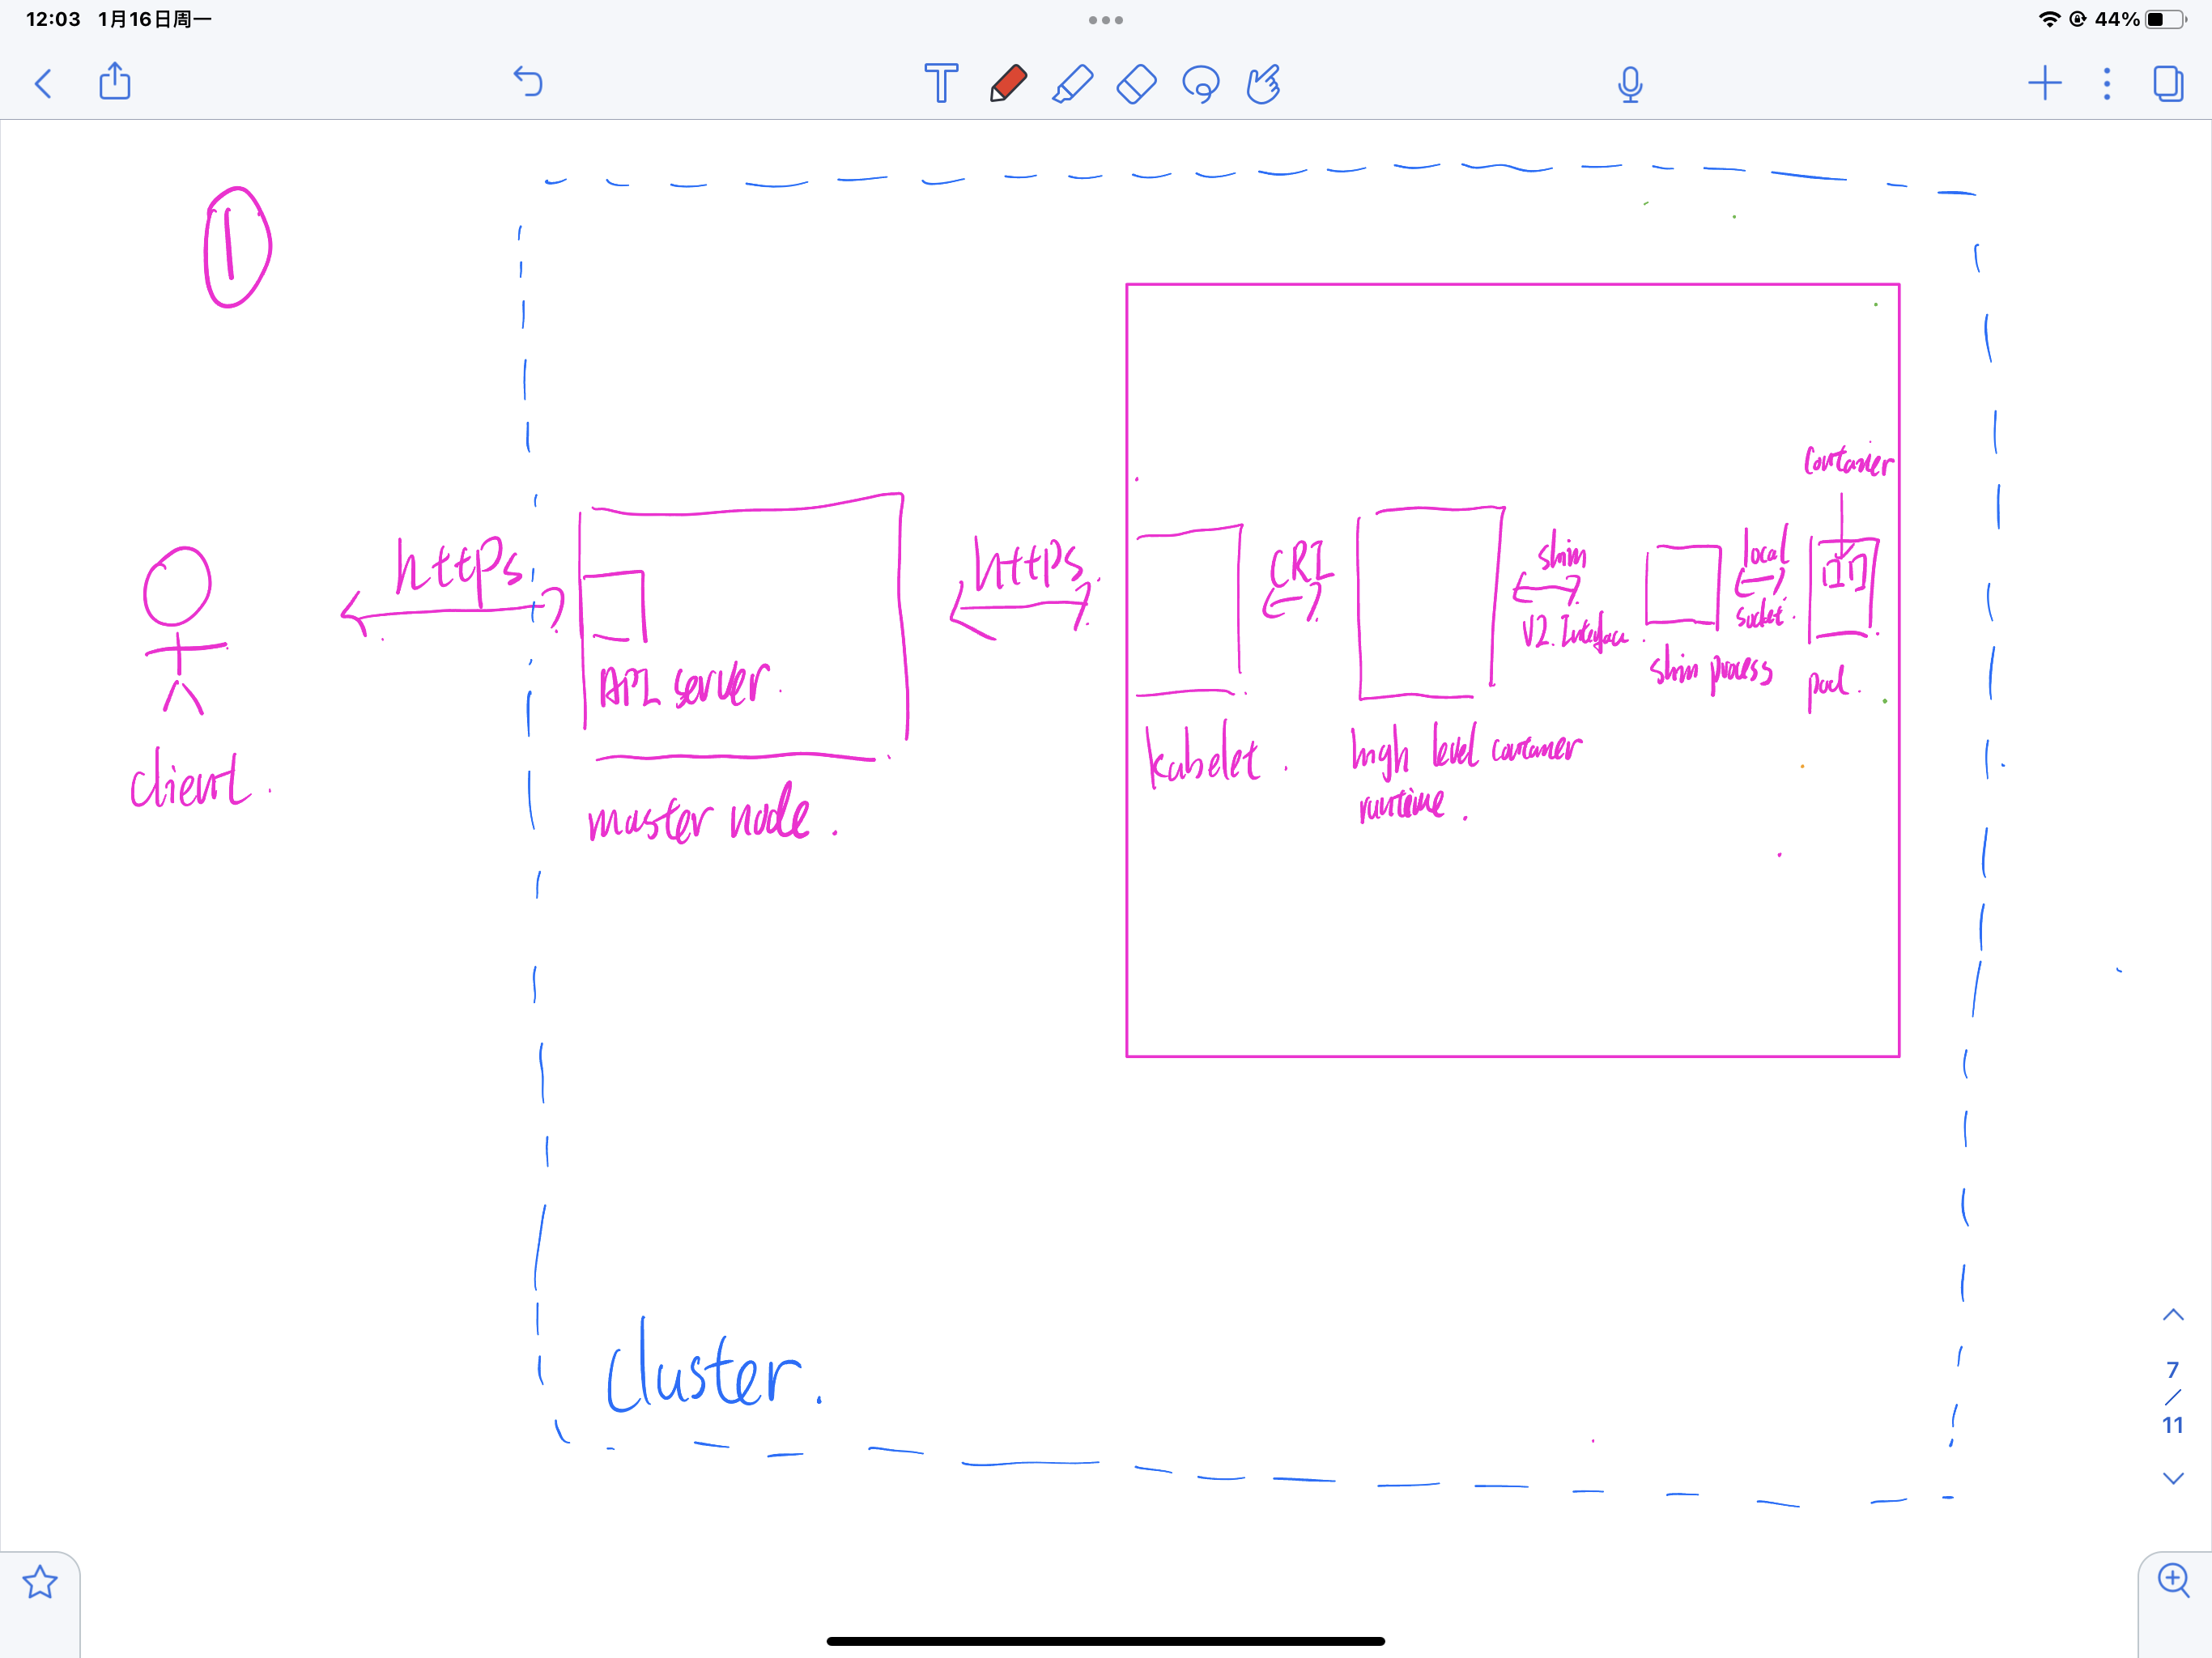
\includegraphics[width=0.8\textwidth]{images/IMG_4416.PNG}
        \caption[k8s arch]{k8s arch}
        \label{fig:k8s}
    \end{figure}

    The tenant connects to the api server located on the master node via the https protocol and issues commands to the cluster via this link
    
    The master node establishes a connection to the kubelet service located on each worker node via the https protocol. Through this link, it can manage the lifecycle of the worker nodes and the pods running on them. Furthermore, commands sent from the tenant to the master node 
    are also sent to the worker nodes through this link, including creating a pod, deleting a pod, etc.
    
    The kubelet at each worker node acts as an agent, listening for requests/commands from the master and calling other services located on the same node to fulfill the request.
    
    In the case of container/image management related requests, it makes a call to a host choosed high level container runtime.
    These High-level container managers, such as containerd, and cri-o, are responsible for managing the container lifecycle and images, while the actual creation/deletion of pods/containers is done by the lower-level container runtime or so called shim process.

    Furthermore, it is worth noting that in order to facilitate communication between kubelet and different high level container runtimes, kubelet proposes an abstract interface called CRI interface. This interface defines a set 
    of endpoints for how high levek container runtime manage the lifecycle of pods/containers and images. Therefore, it must be implemented by any high-level container runtime that wishes to integrate into the k8s environment. This interface breaks the dependency between kubelet 
    and a specific high-level container manager and greatly improves the extensibility of k8s.
    
    Similar to the idea of defining a CRI interface, the high-level container runtime also defines an abstract interface for communicating with shim processes that run containers in different ways. In the case of containerd, this abstract interface is called the shim v2 api. 
    This interface defines endpoints for creating/deleting containers, issuing commands to a container or allocating terminal in a container etc.




    The diagram below shows how containerd works with a kubelet to create a container, where containerd implements the cri interface through the cri plugin


    \begin{figure}[H]
        \centering
        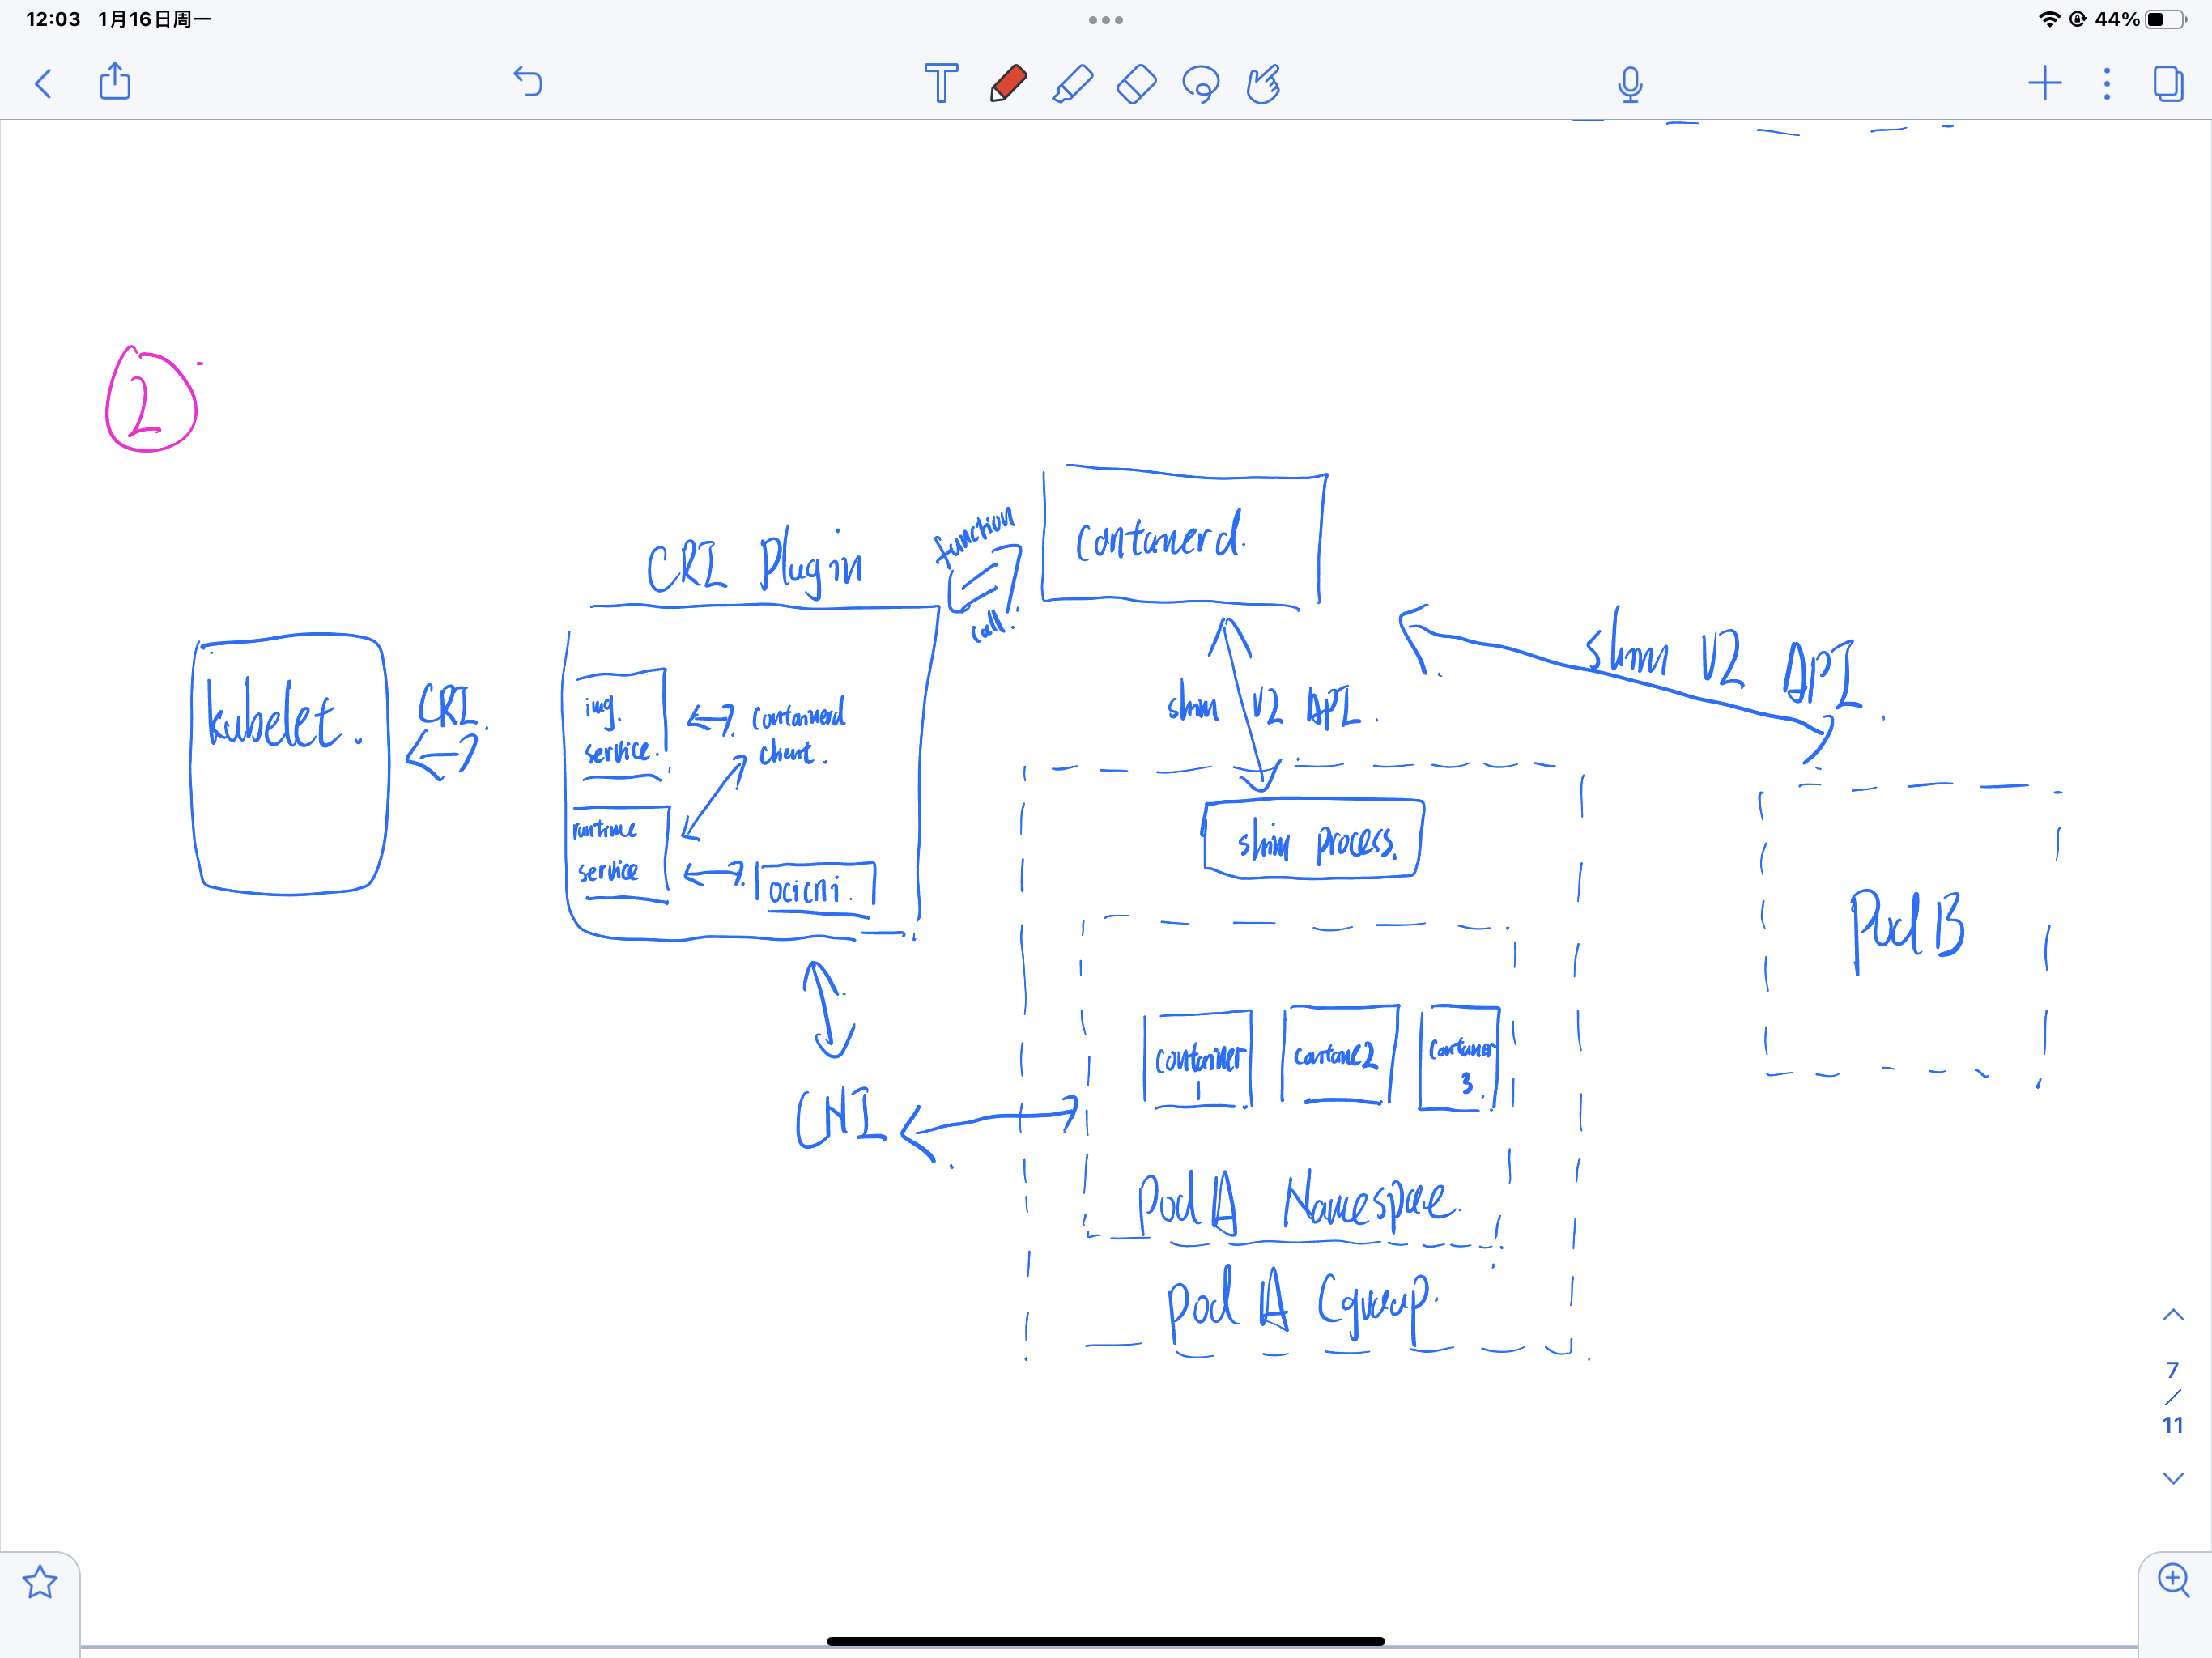
\includegraphics[width=0.8\textwidth]{images/IMG_4417.PNG}
        \caption[Kubelet Workflow]{Kubelet Workflow}
        \label{fig:Kubelet}
    \end{figure}


    \begin{itemize}
        \item Kubelet creates a pod by calling the cri plugin through the CRI Runtime Services API.
        \item The cri plug-in establishes the pod's network namespace, then employ the CNI (Container Network Interface) to configure it;
        \item The cri plugin calls the containerd's function to start a shim process that implements the shim api.
        \item The cri plugin then issues the create and start pod command to the shim process through the shim api, which creates a special pause container as the the sandbox container in the pod's cgroups and namespace.
        \item Kubelet then invokes the cri plug-in through the CRI Image Service API to pull the image for application container.
        \item If there is no image on the local registry, the cri plugin further make use of containerd to pull the image from remote
        \item Kubelet then calls cri plugin , via the CRI runtime service API, to create and start the application container inside the pod using the pulled container image;
        \item Kubelet contacts the cri plugin by using the CRI Runtime Services API to create and launch the application container inside the pod.
        \item cri plugin in turn calls forward those cmds to shim process via shim v2 api.
        \item shim process finally prepaire the container root file system  and loanch the container inside the pod.After these steps, a pod and its corresponding application container is created and running
        \item The shim process finally loads the container root filesystem from a subdirectory of containerd and creates the container in the pod. After these steps, the application container is created and runs in this pod.
    \end{itemize}


\subsection{quark overview}


\begin{figure}[H]
    \centering
    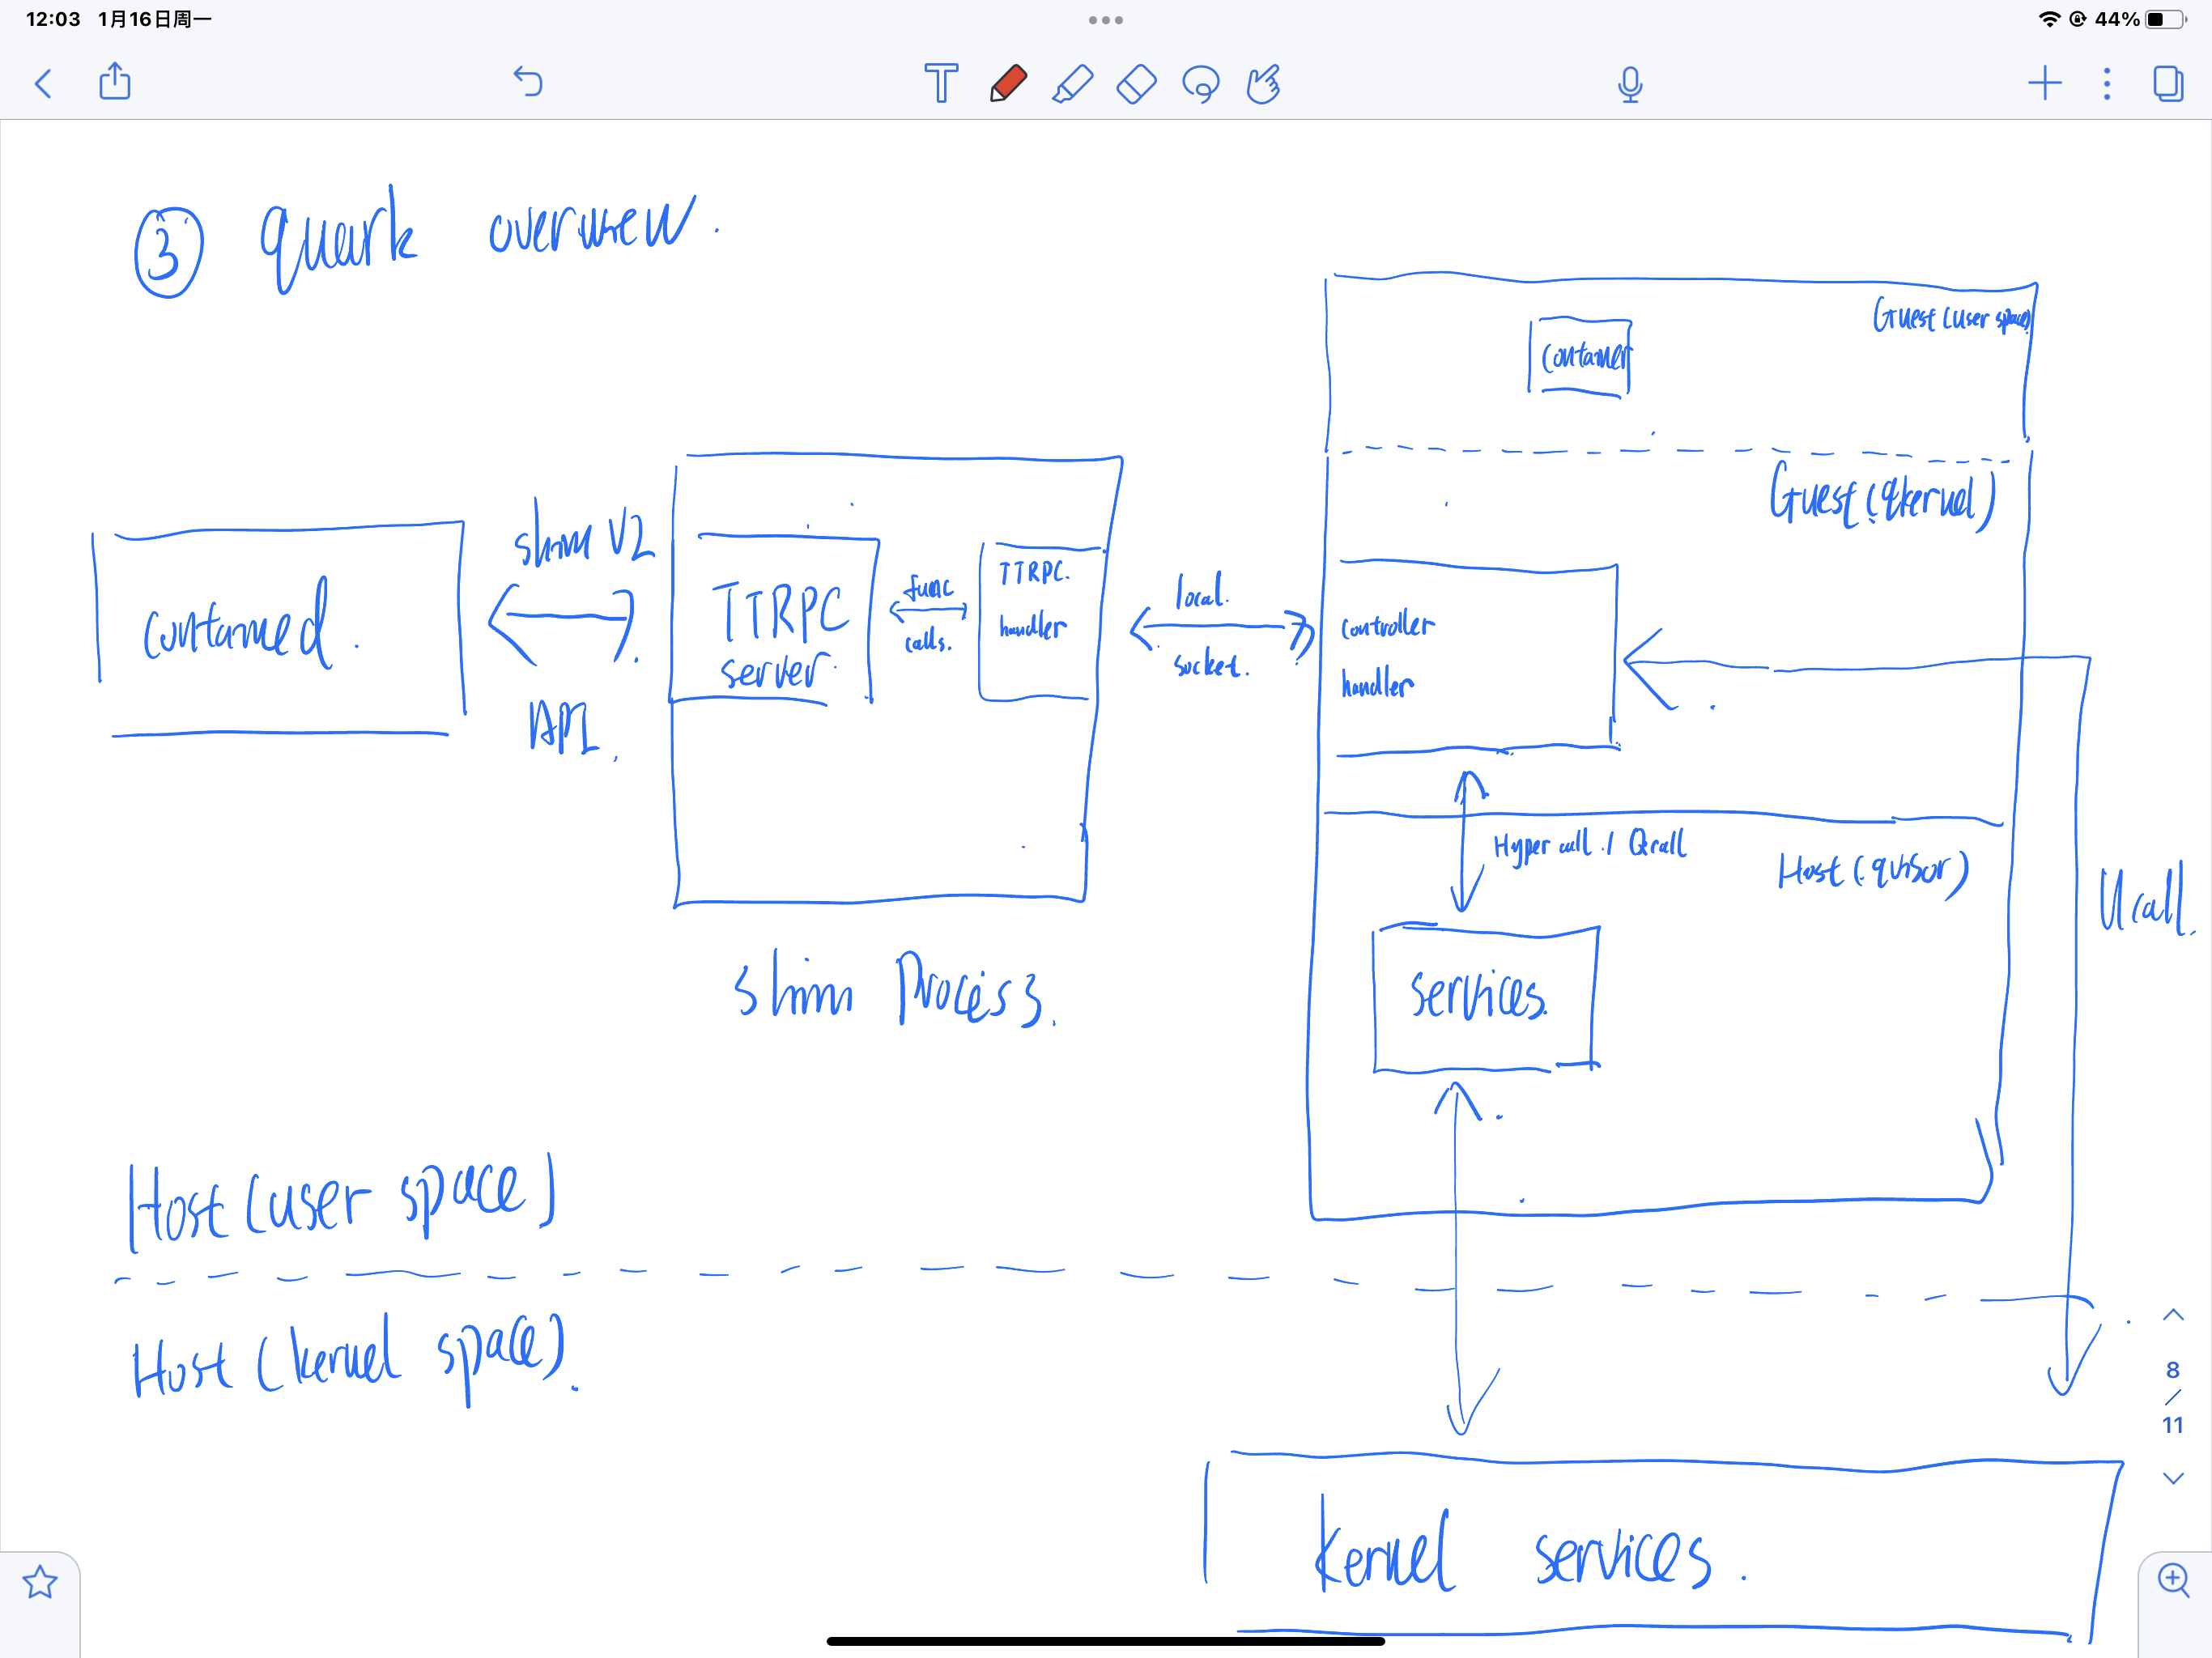
\includegraphics[width=0.8\textwidth]{images/IMG_4415.PNG}
    \caption[quark]{quark}
    \label{fig:quark}
\end{figure}

\subsection{Overview of confidential quark in cloud environments}
\begin{figure}[H]
    \centering
    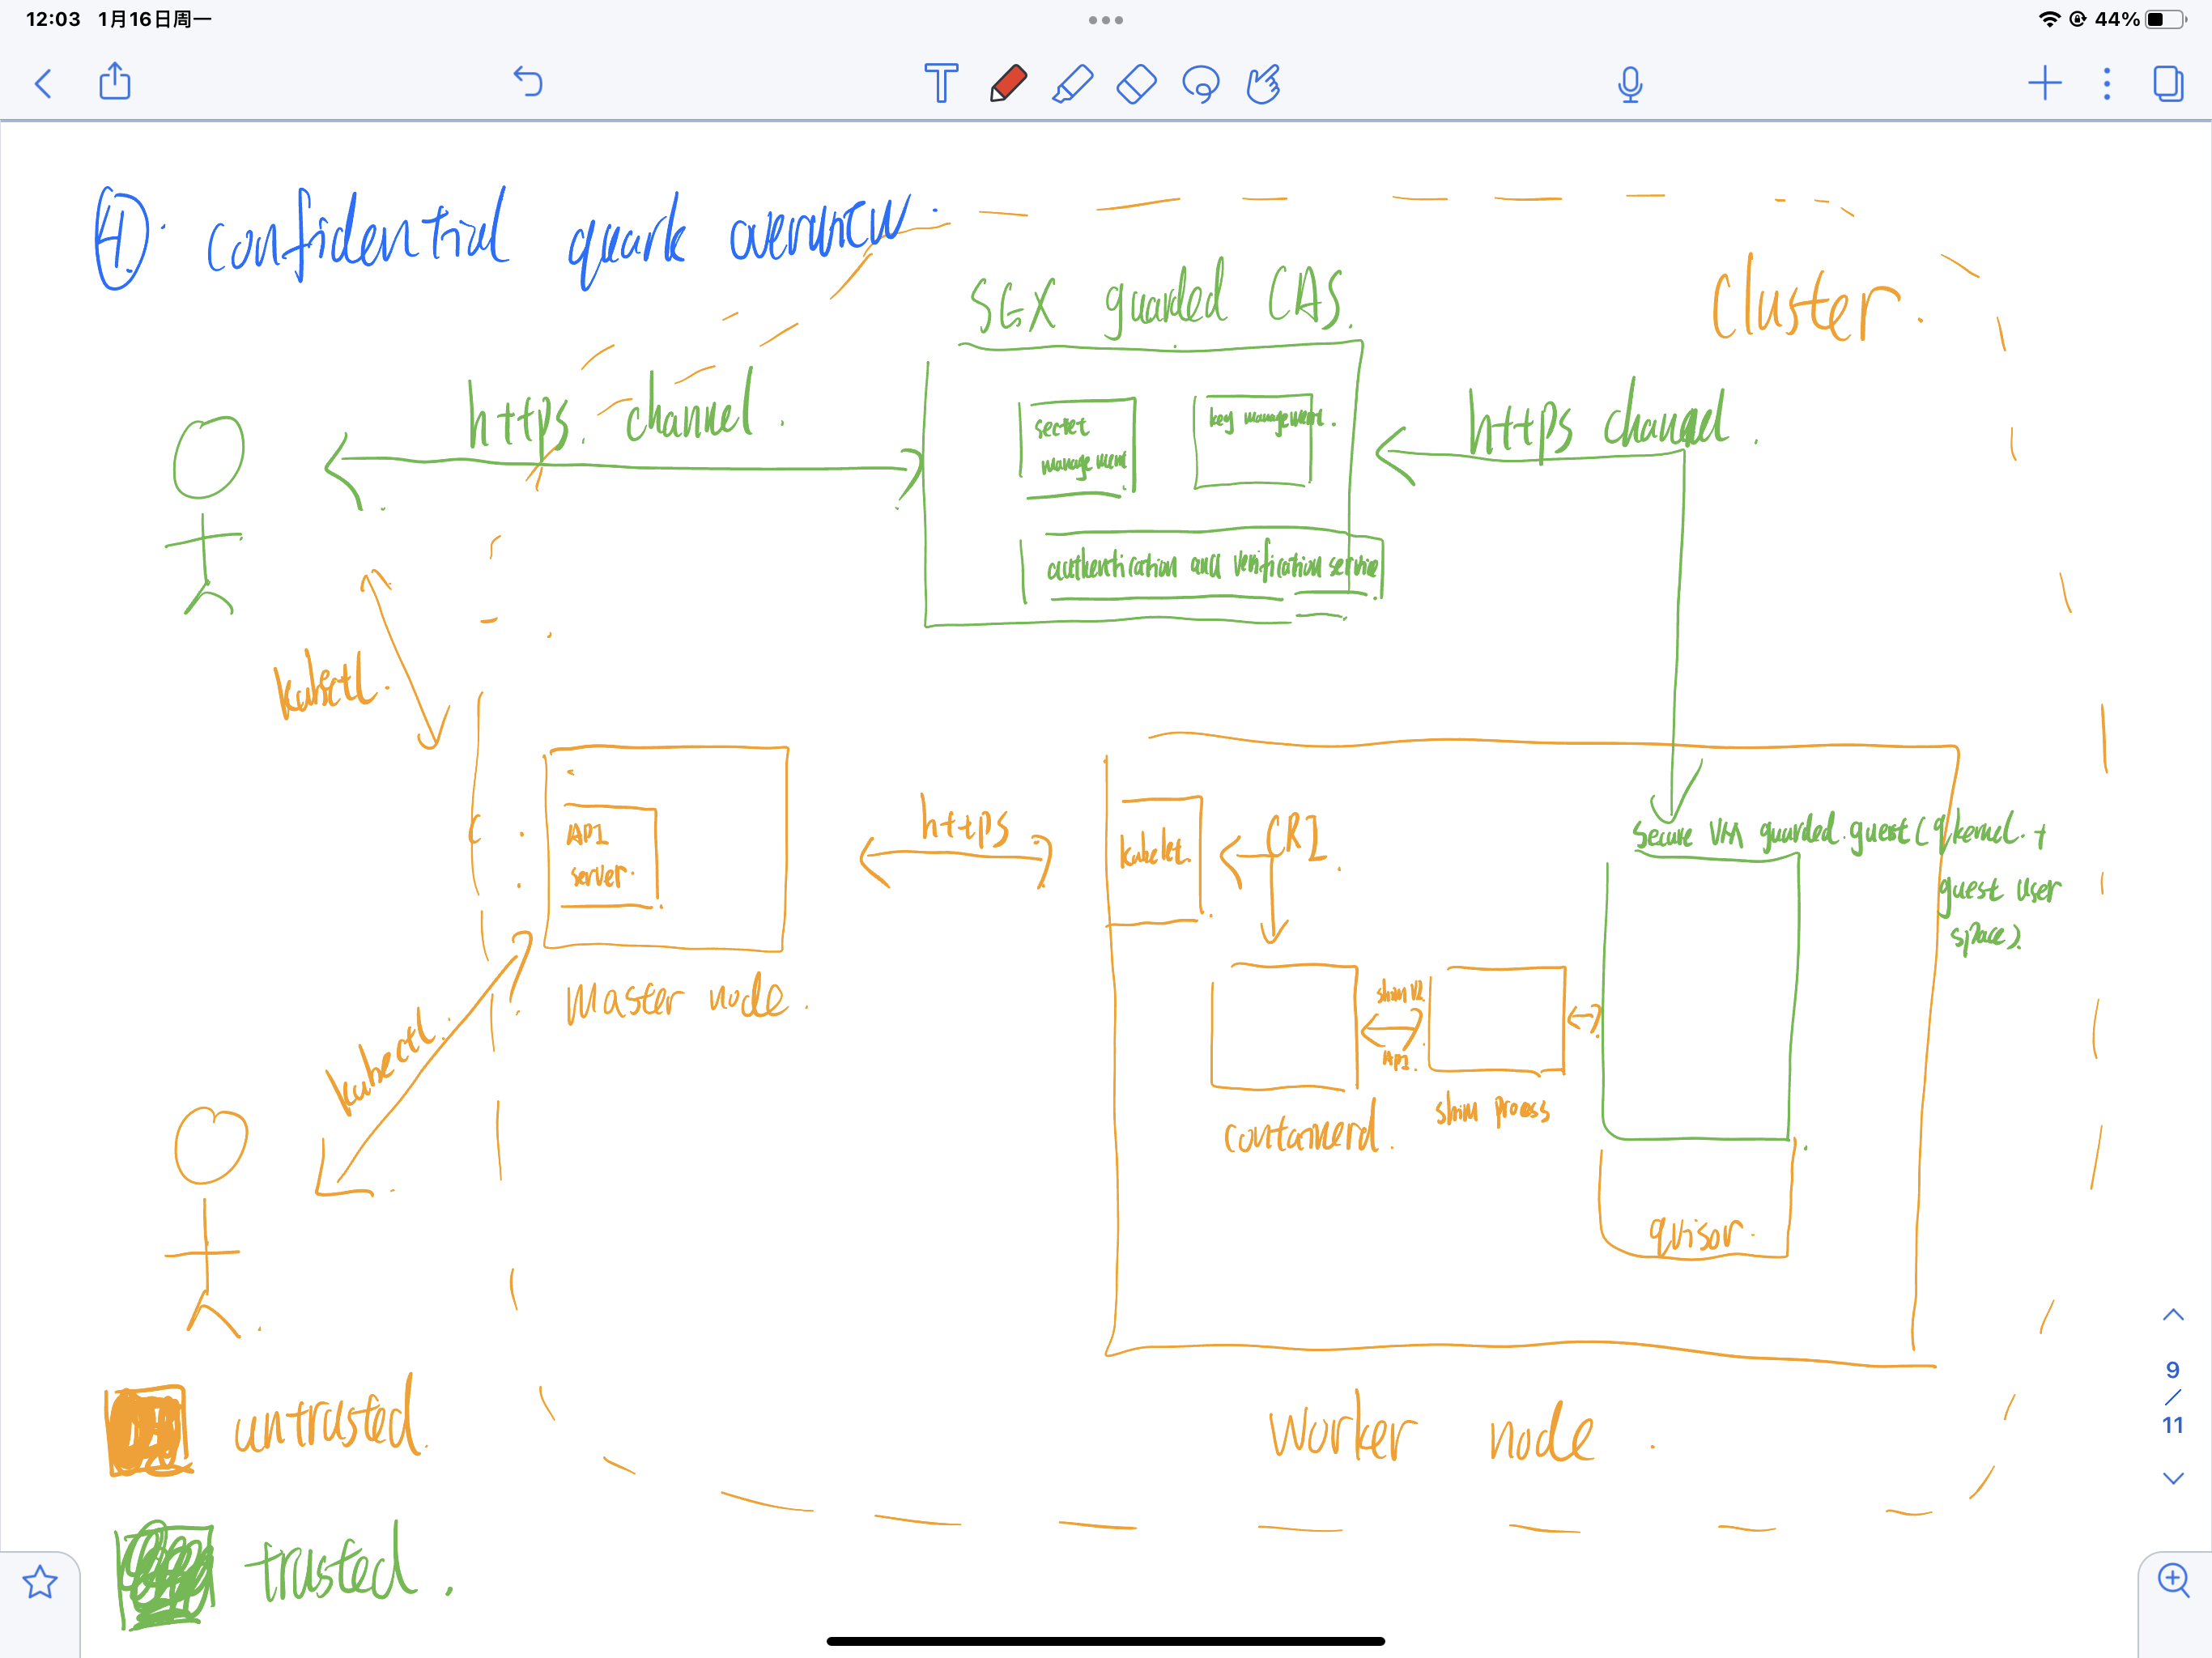
\includegraphics[width=0.8\textwidth]{images/IMG_4414.PNG}
    \caption[confidential quark]{confidential quark}
    \label{fig:confidential_quark}
\end{figure}



\section{Secure deployment(in theory)}

\subsection{How applications obtain secrets?}

Popular applications obtain secrets in three ways
\begin{itemize}
    \item  environment variables
    \item  application arguments
    \item  files.
\end{itemize}

\subsection{How to provide secret to application?}

\begin{itemize}
    \item  The secrets related to environment variables and function arguments are  delivered to the qkernel by a secure channel, after CAS confirms that the qkernel is running in the correct environment through its attestation report
    \item  File-related secrets are encrypted and mounted to a specific location on the container file system.
    \begin{itemize}
        \item After attestation, CAS passes the decryption key to the shield of qkernel.
        \item The shield then load the file, decrypt it and store it in the guest memory before the container starts running.
        \item Any processes in guest that accesses the file always read the plain text version stored in guest memory instead of the encrypted one stored on the host machine
      \end{itemize}
    \item
\end{itemize}

\subsection{How attestation work and how to build the secure channel between CAS and Qkernel}

We use the key brokerage service attestation protocol to establish a communication channel between a Key Broke client (KBC) in secure VM and a trusted Key Broker Service (KBS), 
through which the KBS can verify that the KBC is running in a trusted environment and inject secrets into the KBC in a secure manner.  To support guest attestation and secret injection, the protocol employs the simple, 
and extendable "Request-Challenge-Attestation-Response" (RCAR) method and HTTPS protocol. 

The protocol is divided into two main steps. In the first step, the KBS authenticates the KBC. After the first step is completed, KBS will allow KBCs to request protected resources from it.
Figure from internet:::::::::::::::::::::::

\subsection{The whole procedure}
\begin{itemize}
    \item  The data owner encrypts the file-related secret and prepares the policy for shield running inside the qkernel, where the policy contains the decryption key of the file-related secret, environment variable and arguments-related secret in plaintext
    \item  The data owner attests cas, and uploads the policy if the attestation succeeds.
    \item  The cloud operator then mounts the file-related secrets to the container's file system and starts the container. Note that the IP address of the CAS is passed to the container as an environment variable when the container is started.
    \item  The Shield then starts and sends the POD's attestation report to CAS via https protocol
    \item  CAS verify the attestation report with the help of Intel/AMD remote attestation Infrastructure. If the verification succeeds, CAS sends the policy file to the shield over https channel.
    \item  Shield loads the encrypted file-related secrets from the host, decrypts them, and saves them in the guest's memory. Shield then reads the secrets related to environment variables and application parameters from the policy file and uses them as environment variables and application parameters for the application container process.
\end{itemize}


\section{Runtime issue}
\subsection{Shared library loading during runtime(implement)}
Motivation: Loading malicious libraries during runtime may corrupt the container's confidential execution environment.

Mitigation: Check the libraries' signatures using the signer's public key in the policy file before loading them into guest memory.


\subsection{volume managed by k8s(implement)}
Motivation: Applications that require storage may write their secrets to k8s managed volumes.

Mitigation: 
\begin{figure}[H]
    \centering
    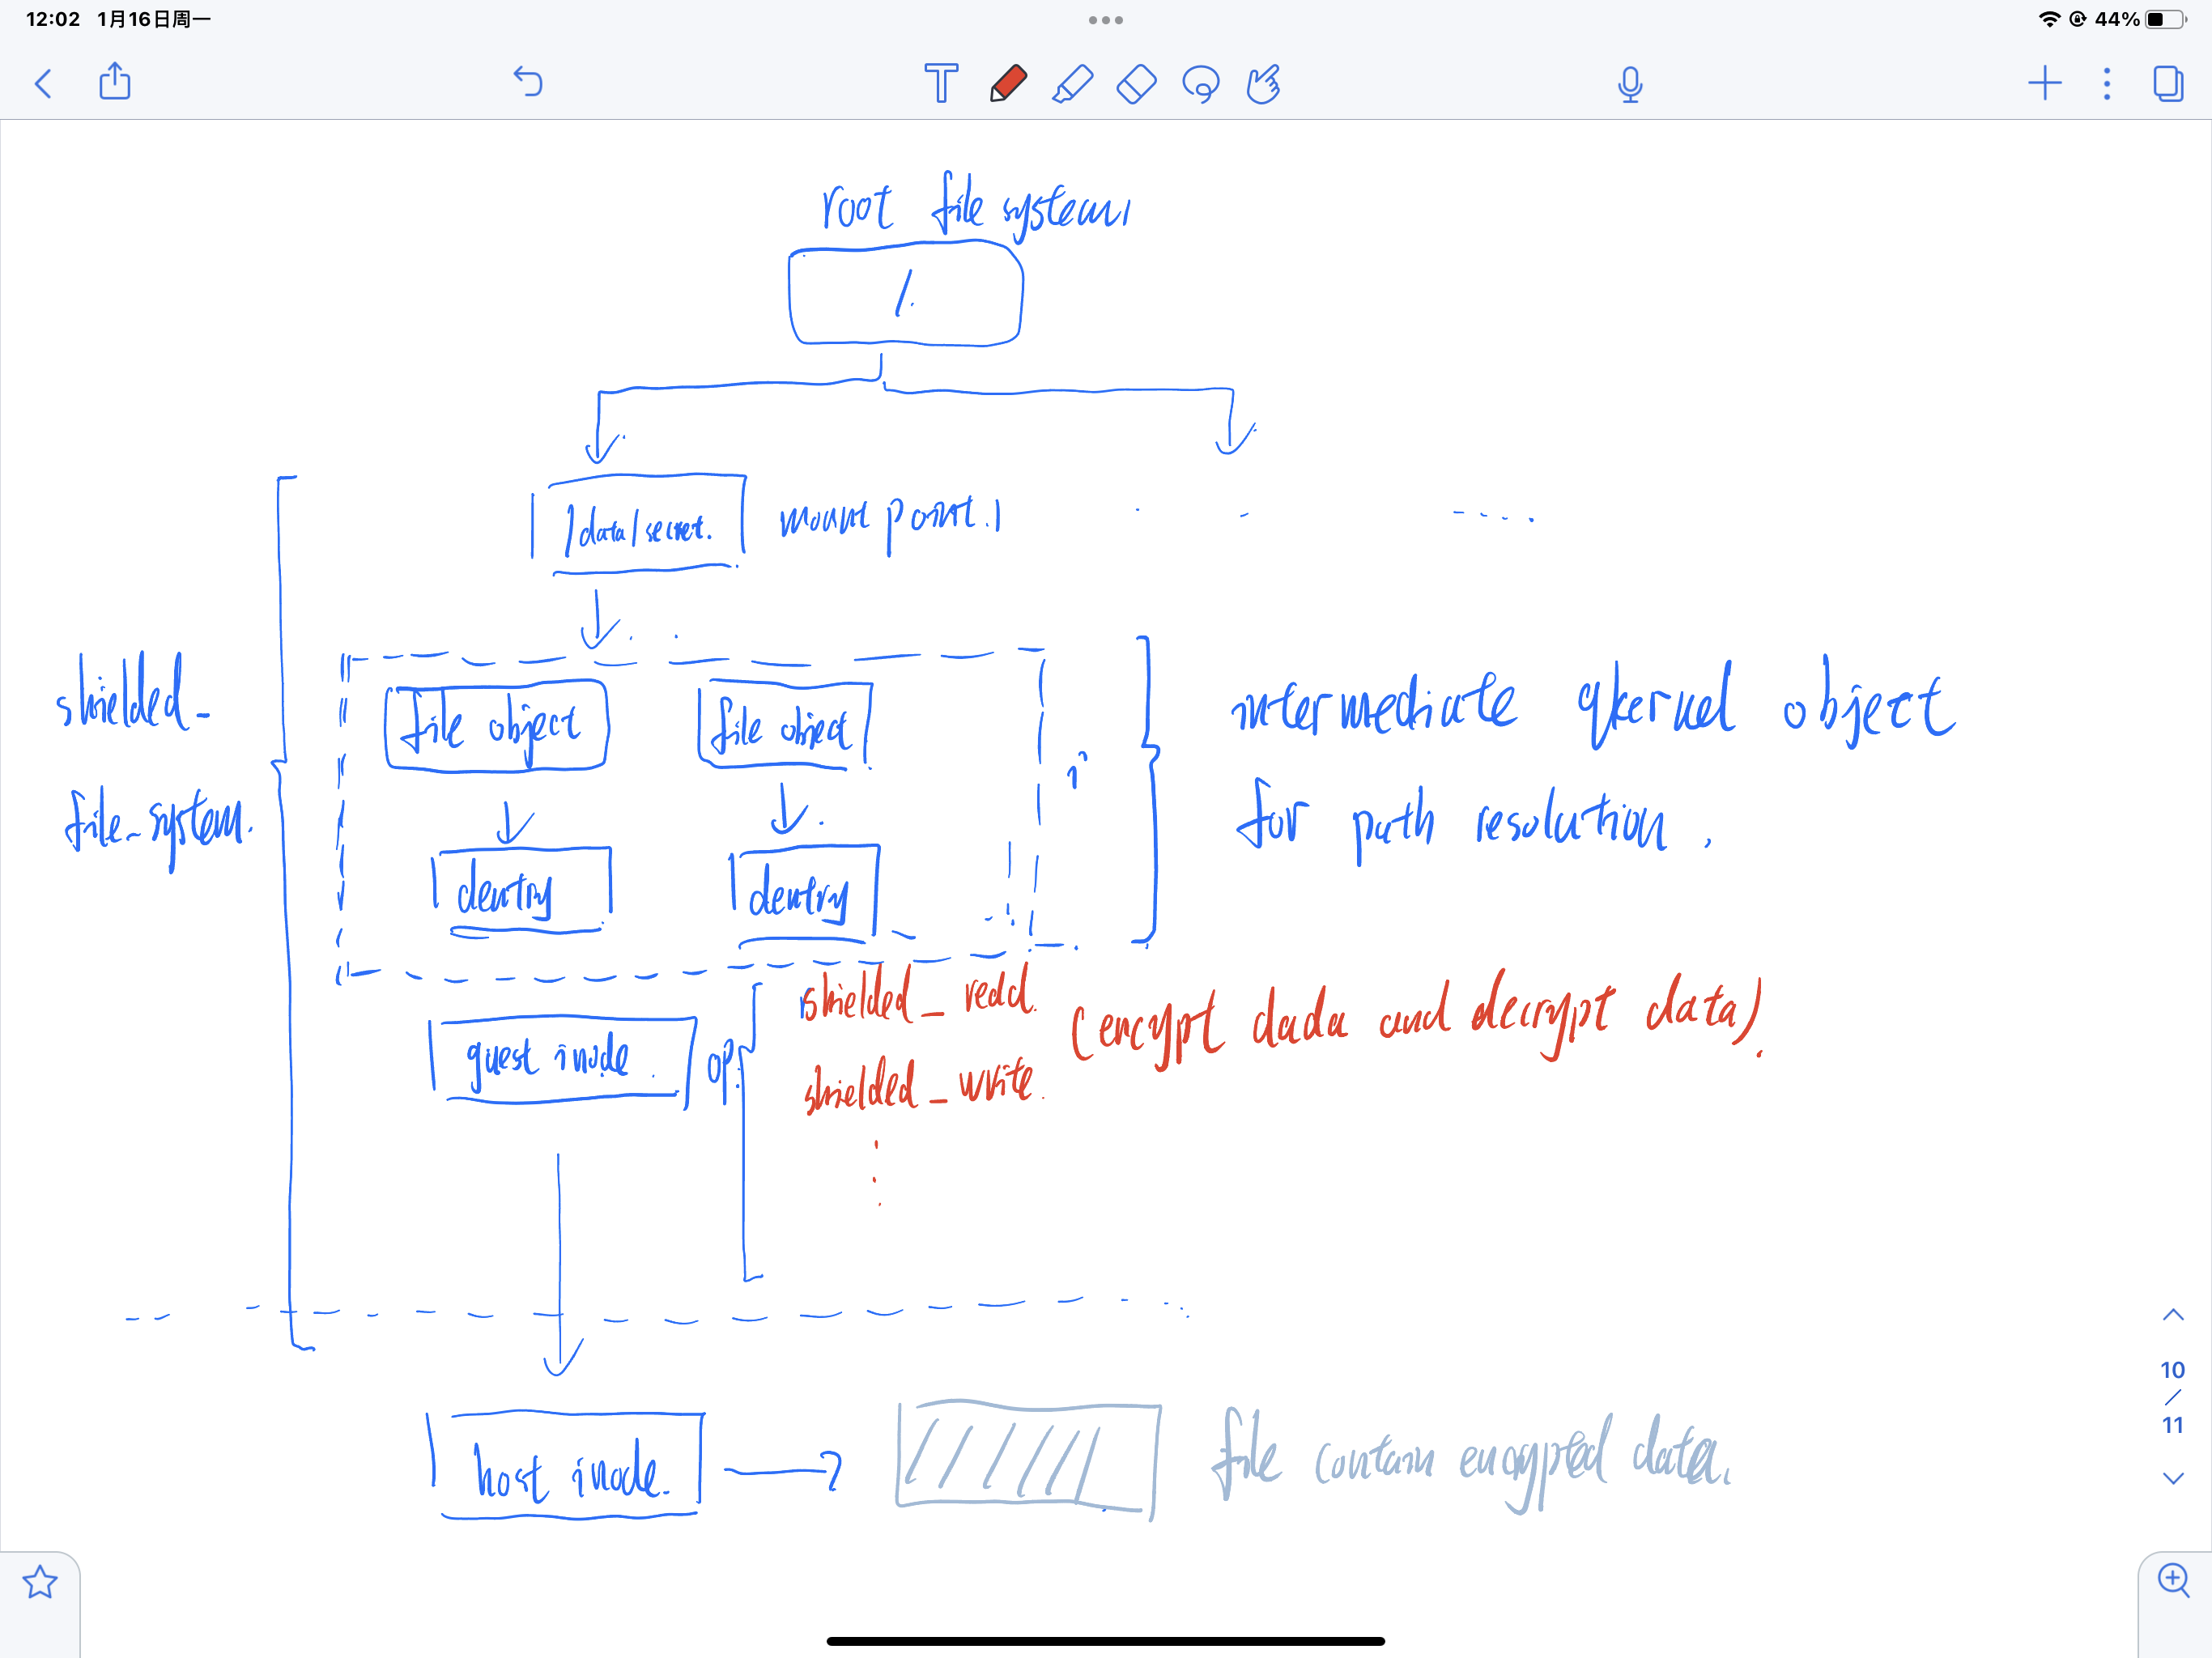
\includegraphics[width=0.8\textwidth]{images/IMG_4413.PNG}
    \caption[shielded file system]{shielded file system}
    \label{fig:shielded_filesystem}
\end{figure}

\begin{figure}[H]
    \centering
    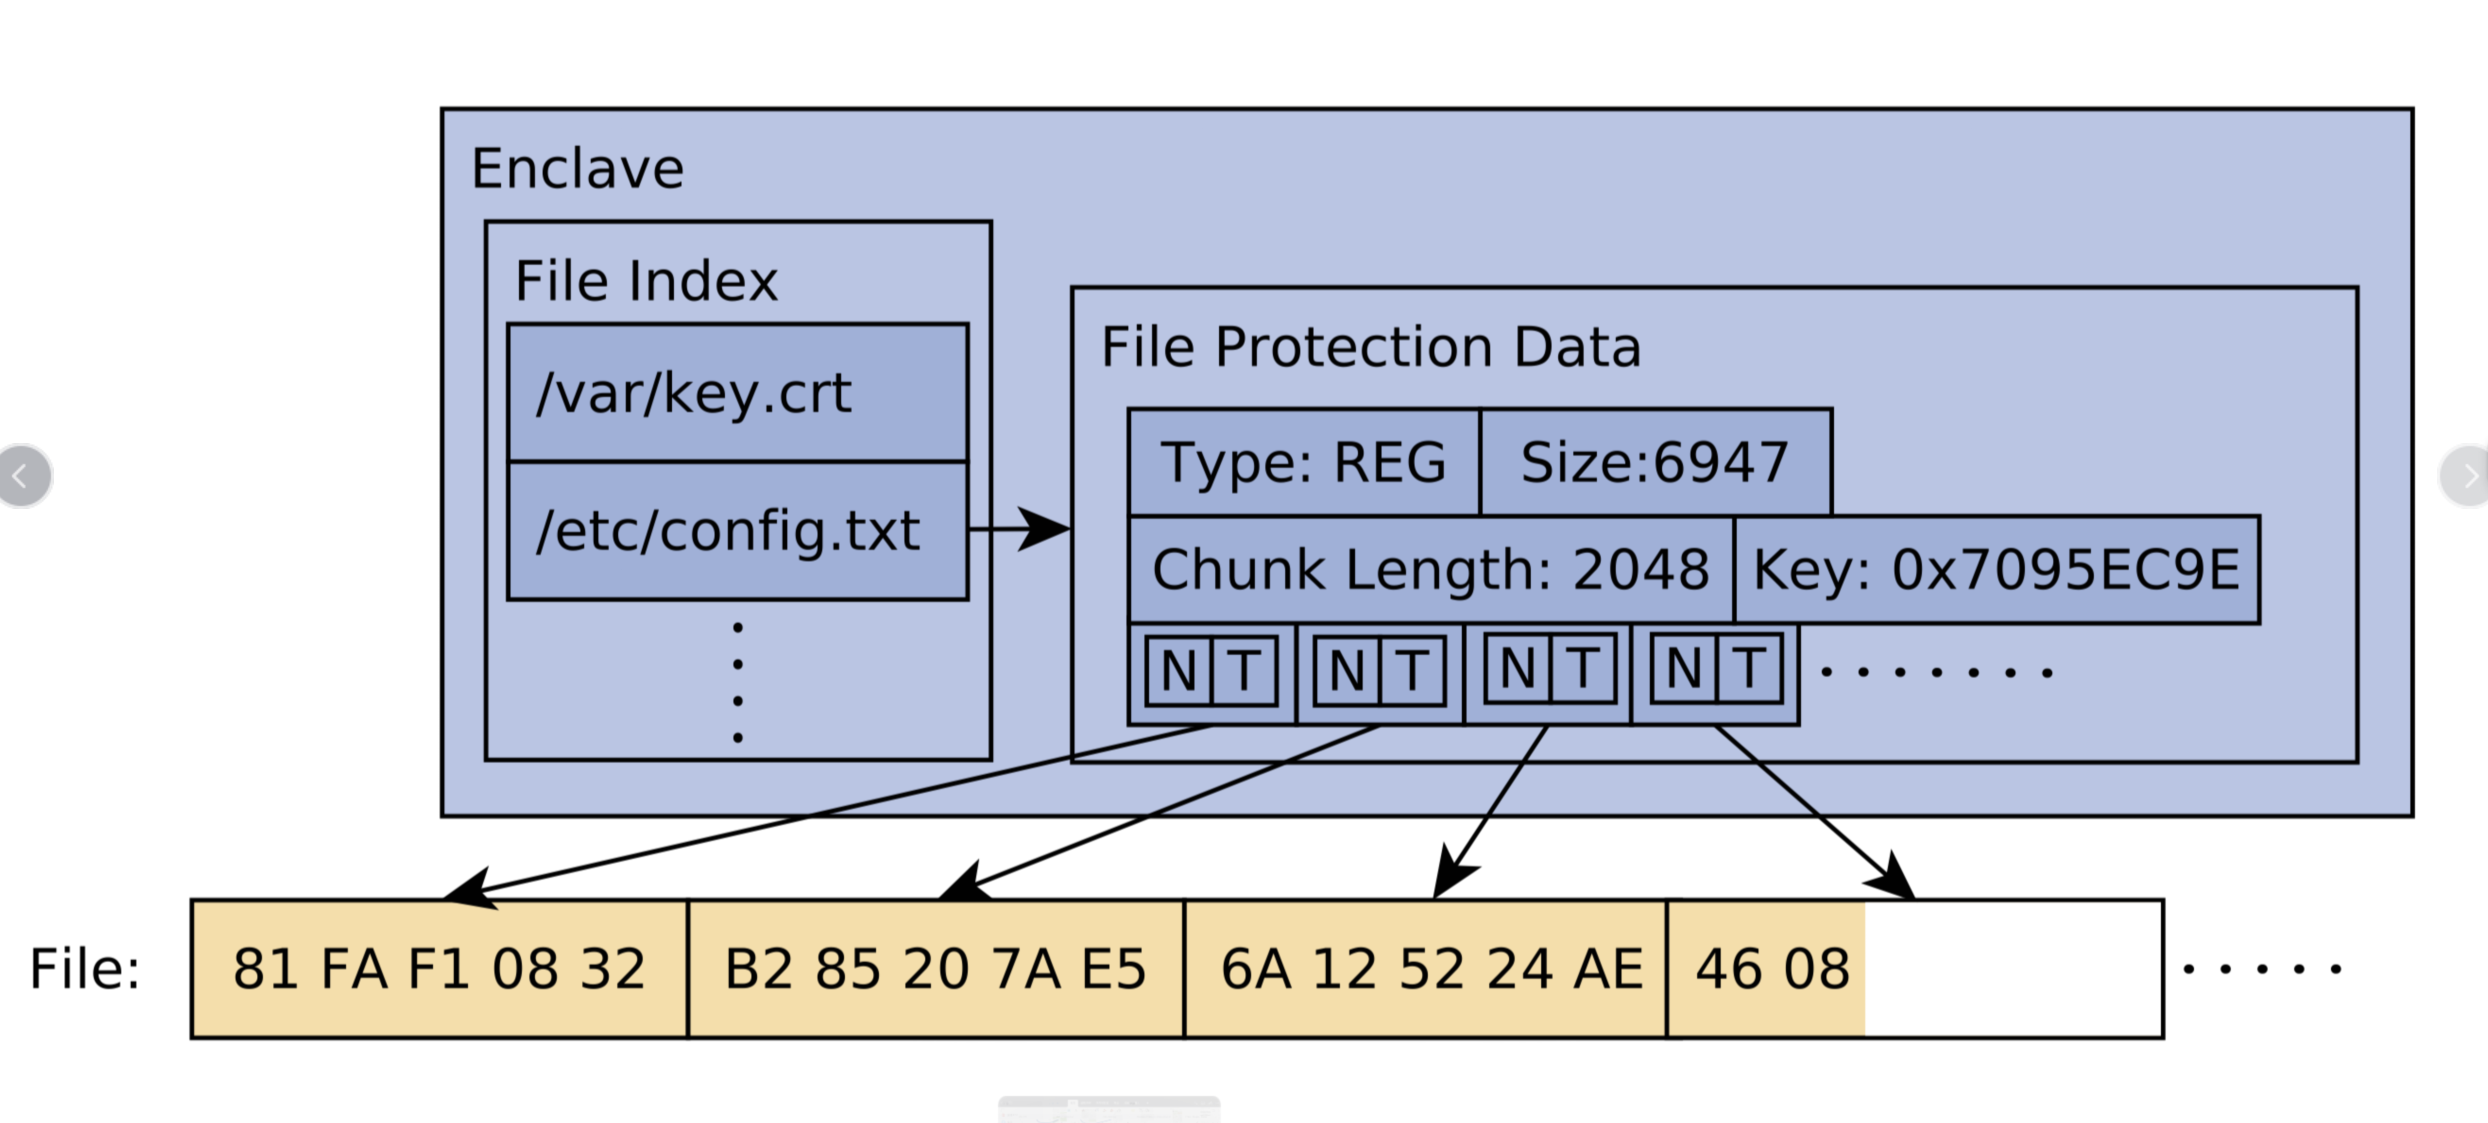
\includegraphics[width=0.8\textwidth]{images/fileencption.png}
    \caption[file content encryption]{file content encryption}
    \label{fig:file_content_encryption}
\end{figure}



\subsection{There may be more issues}
\subsubsection{Shared memory}
\subsubsection{Message queue}

\section{Endpoints related}
\subsection{Overview of endpoints defined in CRI runtime service}
\begin{itemize}
    \item  attach:Attach to a running container
    \item  exec:Run a command/termianl in a running container
    \item  logs: Fetch the logs of a container
    \item  port-forward: Forward local port to a pod

    \item  inspect: Display the status of one or more containers
    \item  inspectp: Display the status of one or more pods
    \item  ps:  List containers
    \item  pods: List pods
    
    \item  create: Create a new container
    \item  start: Start one or more created containers
    \item  run:Run a new container inside a sandbox
    \item  runp:Run a new pod
    \item  rm:Remove one or more containers
    \item  rmp:Remove one or more pods
    \item  stop:Stop one or more running containers
    \item  stopp: Stop one or more running pods

    \item  update: Update one or more running container's resources (CPU, memory etc.)
    \item  stats: List container(s) resource usage statistics
    \item  statsp: List pod resource usage statistics
\end{itemize}

All endpoints can be classified into four categories according to their usage:
\begin{itemize}
    \item  Debug-purpose endpoints:attach, exec, logs, port-forward:
    \item  Endpoints for Pod/container lifecycle management: create, start, run, runp, rm, rmp, stop, stopp
    \item  Endpoints for collecting container/pod metadata stored in high level container runtime: inspect, inspectp, ps, pods
    \item  Endpoints for Pod/container raw resources management (cpu, memory, etc.,): update, stats, statsp
\end{itemize}

\subsection{Exec endpoint}
\subsubsection{Terminal mode(implement)}
Provide option in policy to disable the termianl mode


\subsubsection{Single cmd line mode(implement)}
\subsubsection{How qkenel identify the request issuer}
\begin{itemize}
    \item  cmd issuer first require an access token from CAS, this access token contain the request information and the role of the cmd issuer
    \item  cmd issuer then send the encrypted request along with the access token to qkernel through the k8s channel
    \item  qkernel verifies the token by sending it to CAS. If the token is valid, CAS sends a HTTP response that contains the "true" keyword and other related information
    \item  qkernel finaly exec the cmd according to the policy defined for the role
\end{itemize}
\subsubsection{How to prevent the host from viewing the request contents (cmd and its associate arguments), as well as the request result}
The request itself and its execution results are encrypted and integrity-protected using AES-GCM.

\subsection{Log endpoint (implement)}
Logs streaming from the container's stdout/err are encrypted and integrity-protected using AES-GCM.
\subsection{Attach endpoint}
Since the stdout/err of the container is encrypted, a client without the decryption key cannot get any useful data through the channel established by the Attach endpoint.

\subsection{Port-forward endpoint}
Port-forward endpoint is out of scope

\section{Secure Client(in theory)}

\begin{itemize}
    \item  Prepare the policy and secrets including:
    \begin{itemize}
        \item  encrypts the file-related secrets using key A
        \item requests the cloud operator to mount the encrypted secret to a certain path
        \item embeds key A  and the mount path to policy so that qkernel can find and decrypt it.
        \item  Add arguments and environment variable-related secrets to the policy file
    \end{itemize}
    \item Attest the CAS and upload the policy
    \item  Get access token from CAS, encrypt the Single cmd line mode request, and decrypt its result using the key got from the CAS
    \item  decrypt the container's log using the key got from the CAS
    \item  issue dynamic attestation request to qkernel
\end{itemize}






\cleardoublepage

%%% Local Variables:
%%% TeX-master: "diplom"
%%% End:
